\chapter{\IfLanguageName{dutch}{Stand van zaken}{State of the art}}%
\label{ch:stand-van-zaken}

% Tip: Begin elk hoofdstuk met een paragraaf inleiding die beschrijft hoe
% dit hoofdstuk past binnen het geheel van de bachelorproef. Geef in het
% bijzonder aan wat de link is met het vorige en volgende hoofdstuk.

% Pas na deze inleidende paragraaf komt de eerste sectiehoofding.
VMware~\autocite{vmware} is een bedrijf dat zich specialiseert in virtualisatietechnologieën. De sterke prijsstijgingen van VMware zorgen ervoor dat veel bedrijven afhaken en op zoek gaan naar alternatieven~\autocite{Hale2024}. Er zijn verschillende alternatieve managementplatformen met bijhorende hypervisors.

\subsection{Hypervisors}
In het huidige systeem dat Excentis gebruikt, fungeert VMware ESXi~\autocite{vmware} als onderliggende hypervisor. Deze is closed source en werkt binnen het VMware systeem. Als alternatief voor VMware ESXI zijn er verschillende open-source hypervisors op de markt.
Een voorbeeld hiervan is 'KVM' (Kernel-based Virtual Machine)\autocite{KVM}. KVM is open source en vrij te gebruiken voor iedereen\autocite{KVM}. Microsoft Hyper-V ~\autocite{Eaton2019} wordt ook genoemd als mogelijke vergelijking met VMware ESXI~\autocite{fayyad2013benchmarking}. In dit onderzoek wordt een vergelijking gemaakt tussen verschillende hypervisors die geselecteerd zijn.
Verder in de virtualisatiewereld bestaat ook het Xen Project~\autocite{xenproject}. Dit is een open-source hypervisor die zich vooral richt op cloud computing en server virtualisatie ~\autocite{binu2011virtualization}.
XenServer~\autocite{xenserverwebsite} is ook een alternatieve software keuze voor VMware ESXI. XenServer is een commerciële hypervisor die zich richt op bedrijven en enterprise-ondersteuning biedt.
 
\subsection{managementplatformen}
Excentis gebruikt als managementplatform VMWare vCenter~\autocite{vmware}. Voor dit platform moet een alternatief worden gevonden.
Proxmox VE~\autocite{Proxmox} is een open-source managementplatform dat werkt met KVM en enterprise-ondersteuning aanbiedt voor bedrijven. Uit onderzoek van \textcite{ally2018comparative} blijkt dat Proxmox, dat gebruik maakt van KVM, zeker niet onderdoet tegenover andere closed source systemen.
OpenStack is een open-source cloud computing platform~\autocite{openstack2024}. Deze biedt niet alleen ondersteuning voor KVM maar ook voor Xen~\autocite{oleksiuk2023comparative}.
Microsoft System Center Virtual Machine Manager (SCVMM)~\autocite{microsoftvmm2025} is een product van Microsoft en biedt een managementplatform systeem aan voor Hyper-V.
XenCenter~\autocite{xencenter2024} biedt een managementplatform aan voor XenServer~\autocite{xenserverwebsite}.

\subsection{Open source systemen}
Er zijn vele soorten softwarepakketten op de markt die hypervisors en managementplatformen aanbieden. Bij het bekijken van de verschillende managementplatformen met hun bijbehorende hypervisors kunnen deze worden onderverdeeld in twee groepen: de closed-source en open-source hypervisors. Elke groep heeft zijn voor- en nadelen. Alles hangt steeds af van de noden en vereisten van het bedrijf of instelling.
Proxmox VE is open source~\autocite{Proxmox}. Dit wil zeggen dat de systemen kosteloos gebruikt kunnen worden. Support bij problemen valt hierbij wel af. Er is wel een mogelijkheid om bij hen een enterprise support services subscription te nemen. Hierbij kan er alsnog beroep worden gedaan op support bij eventuele problemen.
Open source software is een evidentie maar zorgt voor meer zelfstandig werk bij installatie en rust meer op de community achter de software.

\subsection{closed source systemen}
Andere alternatieven zijn closed-source. Hierbij gaat het onder andere om VMware ESXi/VMware vCenter~\autocite{vmware} en Microsoft Hyper-V~\autocite{Eaton2019}. Deze software systemen zijn niet gratis en vragen een licentie om te mogen gebruiken. Dit is een nadeel ten opzichte van open-source systemen.
Bij bedrijven waar stabiliteit en betrouwbaarheid hoog in het vaandel staan, zoals in een wetenschappelijke omgeving met supercomputers die veel geld kosten als ze niet draaien, kan het een goede keuze zijn om te kiezen voor closed-source hypervisors~\autocite{voras2012early}. Dit wil niet zeggen dat andere systemen uitgesloten zijn.
\subsection{Soorten storage systemen}
Wanneer het over opslag in de virtualisatiewereld gaat, betreft het ook 'Serial-Attached SCSI' (SAS) en 'Direct-Attached Storage' (DAS). Deze technologieën zorgen ervoor dat er een hoge beschikbaarheid is van de data en dat deze snel kan worden opgevraagd~\autocite{griswold2002storage}. Dit is een belangrijk aspect in de virtualisatiewereld en is belangrijk voor Excentis dat deze beide technologieën perfect werken en ondersteunt worden.
SAS is een snelle, betrouwbare opslaginterface die servers en high-performance opslagapparaten verbindt~\autocite{aravindan2014performance}. Dit is een belangrijk om een consistente opslag te garanderen. DAS is een opslagarchitectuur waarbij opslag direct fysiek is verbonden aan een enkele server, zonder tussenkomst van een netwerk. Deze technologie is goedkoper en eenvoudiger, maar garandeert niet alle voordelen die SAS wel kan garanderen~\autocite{griswold2002storage}.
DAS wordt vaak gebruikt in kleinere bedrijven waar de data niet zo belangrijk is en waar de data niet zo vaak wordt opgevraagd. SAS wordt vaak gebruikt in grotere bedrijven waar de data zeer belangrijk is en waar de data vaak wordt opgevraagd~\autocite{griswold2002storage}.
Zo goed als alle managementplatformen ondersteunen DAS en SAS in ons onderzoek. Excentis wilt weten hoe deze ondersteuning kan worden overgezet naar een nieuw managementplatform.

\subsection{High Availability-ondersteuning}
In het onderzoek van~\textcite{dudnik2017creating} wordt een grote vergelijking gemaakt tussen hypervisors en hun managementplatformen. Hierin wordt gefocust op bepaalde aspecten binnen de term High Availability, zoals redundantie, risicoanalyse en piekdrukte.
Er zijn verschillende aspecten die moeten worden bekeken en waaraan voldaan moet worden om aan een goede High Availability te voldoen. Een failover-systeem dat het ene systeem het andere systeem over laat nemen bij een bepaalde fout, is een van die aspecten.
Op netwerkniveau moet er ook nagedacht worden over zowel schaalbaarheid bij piekmomenten als bij problemen die zich voordoen in het netwerk. Migratie tussen verschillende fysieke servers moet ook mogelijk zijn om een goede High Availability te garanderen~\autocite{dudnik2017creating}.
Workloadmanagers kunnen een goede oplossing zijn om overbelasting tegen te gaan op drukke piekmomenten. Back-ups van de data worden ook gezien als een belangrijk aspect voor High Availability.


\subsection{samenvatting van alle managementplatformen en hun bijhorende hypervisors}
    \begin{table}[h!]
        \centering
        \begin{tabular}{|l|l|l|l|}
        \hline
        \textbf{Platform}      & \textbf{Type}      & \textbf{Hypervisor} & \textbf{Description} \\ \hline
        VMware vCenter         & Closed-source      & VMware ESXi         & Enterprise management platform voor VMware-gebaseerde virtualisatie. \\ \hline
        Microsoft SCVMM        & Closed-source      & Microsoft Hyper-V   & Beheert Hyper-V-omgevingen en biedt integratie met andere Microsoft-producten. \\ \hline
        Proxmox VE             & Open-source        & KVM                 & Geavanceerd open-source managementplatform voor KVM, met enterprise-ondersteuning. \\ \hline
        OpenStack              & Open-source        & KVM, Xen            & Cloud computing-platform dat meerdere hypervisors ondersteunt. \\ \hline
        XenCenter              & Closed-source      & XenServer           & Managementplatform specifiek ontworpen voor XenServer-gebruikers. \\ \hline
        Xen Project            & Open-source        & Xen                 & Managementplatform dat Open-source is. \\ \hline
        \end{tabular}
        \caption{Vergelijking van Virtualisatieplatforms}
        \end{table}
        
\subsection{Prestatie verschillen tussen XenServer en Proxmox VE}
In het onderzoek van \textcite{algarni2018performance} wordt een vergelijkende studie gemaakt tussen Xen en KVM. In ons onderzoek focussen wij ons vooral op het managementplatform.
Aangezien een managementplatform ook een hypervisor nodig heeft kunnen wij hier spreken over het management platform die gekoppeld is in deze studie aan een hypervisor.
Voor KVM spreken we over PROXMOX VE en voor Xen spreken we over XenServer. In deze studie wordt er een vergelijking gemaakt tussen de twee systemen en hun prestaties. De resultaten zijn als volgt:
\begin{itemize}
    \item Proxmox VE heeft een betere prestatie in termen van CPU-gebruik en geheugengebruik dan XenServer.
    \item XenServer heeft een betere prestatie in termen van I/O-prestaties dan Proxmox VE zoals bestandssysteem beheer en applicatie prestaties.
\end{itemize}                               
Over het volledige onderzoek van \textcite{algarni2018performance} heen krijg KVM (gekoppeld aan Proxmox VE voor ons onderzoek) de beste punten over het globael punt heen. Dit onderozek heeft plaats gevonden in 2018 waarbij de conclusies nog alst actueel kunnen beschouwd worden.
Dit is een belangrijk onderzoek om conclusies uit te trekken eenmaal een proof of concept gemaakt is.

\subsection{Storage ondersteuning voor hypervisors en managementplatformen}
Zoals eerder uitgelegd wordt er in dit onderzoek gekeken naar Serial-Attached SCSI (SAS) en Direct-Attached Storage (DAS). Deze technologieën zijn belangrijk voor de virtualisatiewereld en zijn ook belangrijk voor Excentis. Het is belangrijk dat deze technologieën goed werken met de hypervisors en managementplatformen die in dit onderzoek worden bekeken.
Om in de proof of concept deze technologieën te kunnen gebruiken moet er gekken worden of elk managamentplatform deze technologieën ondersteunt.
SAS storage staat los van elke hypervisor met hun bijhoren virtual managementplatformen. 
\begin{figure}[h!]
    \centering
    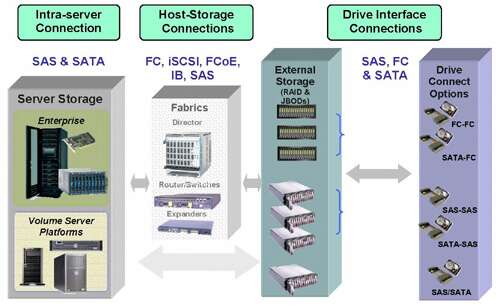
\includegraphics[width=0.7\textwidth]{../onderzoek/storagesas-das.jpg} 
    \caption{volledig beeld die SAS weergeeft, afkomstig van \href{https://www.eetimes.com/serial-attached-scsi-storage-moves-ahead-in-network-server-designs/}{TechTarget}.}
    \label{fig:sas}
\end{figure}
De onderstaande figuur toont de kracht van SAS systemen. In het artikel van \textcite{loshin2022sas} wordt er uitgelegd dat SAS tot 2 keer zoveel meer data kan versturen en verwerken t.o.v. het bekende SATA systeem.
\begin{figure}[h!]
    \centering
    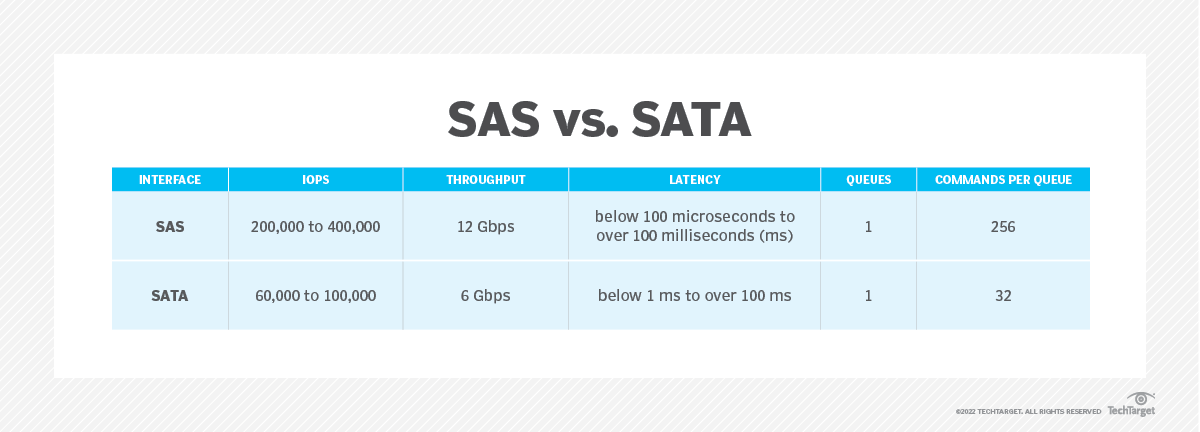
\includegraphics[width=0.7\textwidth]{../onderzoek/sas_vs_sata-f.png} 
    \caption{Afbeelding die SAS prestatie weergeeft, afkomstig van \href{https://www.techtarget.com/searchstorage/definition/serial-attached-SCSI}{TechTarget} over Serial Attached SCSI.}
    \label{fig:sas}
\end{figure}


Bij DAS-systemen wordt, zoals eerder vermeld, de data rechtstreeks aan de hardware verbonden. Het onderzoek van \textcite{joshi2014empirical} richt zich specifiek tot schijfformaten op DAS-systemen.
Dit gaat buiten de scope van dit onderzoek, maar toont zeer mooi aan dat KVM (voor ons Proxmox VE) zeer goede ondersteuning biedt en hierbij ook aantoont dat er zeer veel ondersteunende schijfformaten bestaan.
Het is zeer moeilijk om correcte wetenschappelijke artikels te vinden over implementatie van DAS- en SAS-systemen op alle soorten managementplatformen. Er wordt vaak specifiek gericht op een gebruikt systeem die zich onder de categorie bevindt DAS of SAS. Het onderzoek van \textcite{joshi2014empirical} is daar een goed voorbeeld van.
Met de referenties en kennis die hieruit zijn gekomen, weten we dat DAS en SAS globaal over alle managementplatformen ondersteund worden. De uitvoering en de praktische ervaring zal in de proof of concept worden bekeken. Daaruit moet uitkomen of de SAS- en DAS-integratie voldoende stabiliteit biedt.

\begin{figure}[h!]
    \centering
    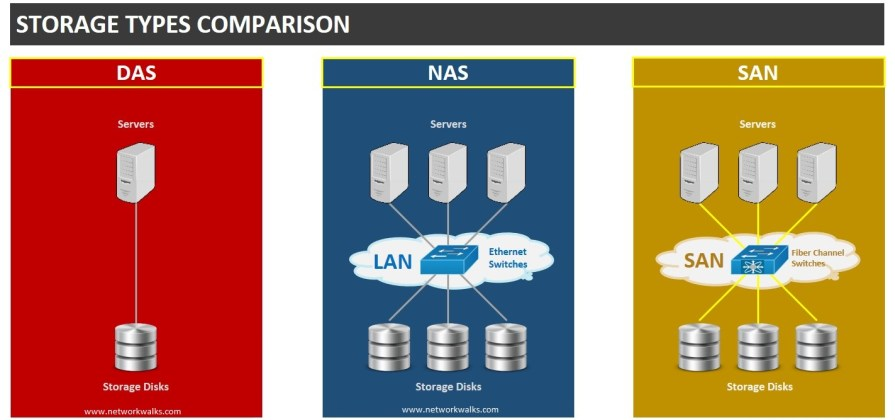
\includegraphics[width=0.7\textwidth]{../onderzoek/DAS.jpg} 
    \caption{Afbeelding die DAS simpel weergeeft, afkomstig van \href{https://networkwalks.com/storage-types-das-nas-san/I}{TechTarget}.}
    \label{fig:sas}
\end{figure}